\section{Appunti  Thu 23 May 2019 02:46:13 PM CEST}
\begin{figure}[ht]
    \centering
    \begin{circuitikz}
        \draw(-1, 3) node[nmos] (N1){};
        \draw(1, 3) node[nmos, xscale=-1] (N2){};
        \draw(N1.G) to[short, -o] ++ (-0.2, 0) node[above]{$V_1$};

        \draw (0, 0) node[eground] (G){}
        to[isource, -*] ++ (0, 2) node(bisection){$V_x$} -- ++ (-1, 0) -- (N1.S);
        \draw (N1.D) to[short, -o] ++ (0.5, 0)
            node[above]{$V_{U1}$};

        \draw(1.2, 1) node[anchor=east]{$\big\uparrow I_0$};
        \draw(N1.D) to[R, -o] ++(0, 2)
            -- ++ (0, 1)
            -- ++ (1, 0)
            node(UB){}
            -- ++ (1, 0)
            -- ++ (0, -1)
            to[R, o-*] (N2.D);

        \draw(bisection.center) -- ++ (1,0) -- (N2.S);
        \draw(N2.G) to[short, -o] ++ (0.2, 0) node[above]{$V_2$};
        \draw(N2.D) node[right]{$V_{U2}$};

        \draw(UB.center) to[short, ->] ++ (0, 1) node[vdd]{$V_{DD}$};
    \end{circuitikz}
    \caption{Amplificatore Differenziale\label{amp_diff}}
\end{figure}


\[
    \begin{cases}
        V_{id} = V_1 - V_2\\
        V_{ic} = \frac{V_1 + V_2}{2}
    \end{cases}
\]

\section{Amplificatore Operazionale}
\begin{minipage}{0.45\textwidth}
\begin{circuitikz}
    \draw(0, 0) node[above]{$V_{U2}$} to[short, *-] (1, 0) node[not port, anchor=in](np){};
    \draw(np.out) to[short, -*] ++(1, 0) node[above] {$V_{U2}^{1}$} ;
\end{circuitikz}
\end{minipage}
\begin{minipage}{0.45\textwidth}
\begin{figure}[H]
    \centering
    \begin{tikzpicture}
        \begin{axis}[
            xmin=0,
            xmax=6,
            axis lines = middle,
            ymax=4,
            yticklabel=\empty,
            xlabel=$V_u$,
            ylabel=$V_u^1$,
            xticklabels={$V_{DP}$,$V_{DD}$},
            xtick={1,3}
            ]
            \addplot[color=red, domain=-4:1]{3};
            \addplot[color=red, domain=1:3]
                { 3*exp(-(x-1)^2)};
            \addplot[color=red, domain=3:10]{3*exp(-4)};
            \addplot[mark=none, dashed] coordinates{(1, 0) (1, 3)};
        \end{axis}
    \end{tikzpicture}
    %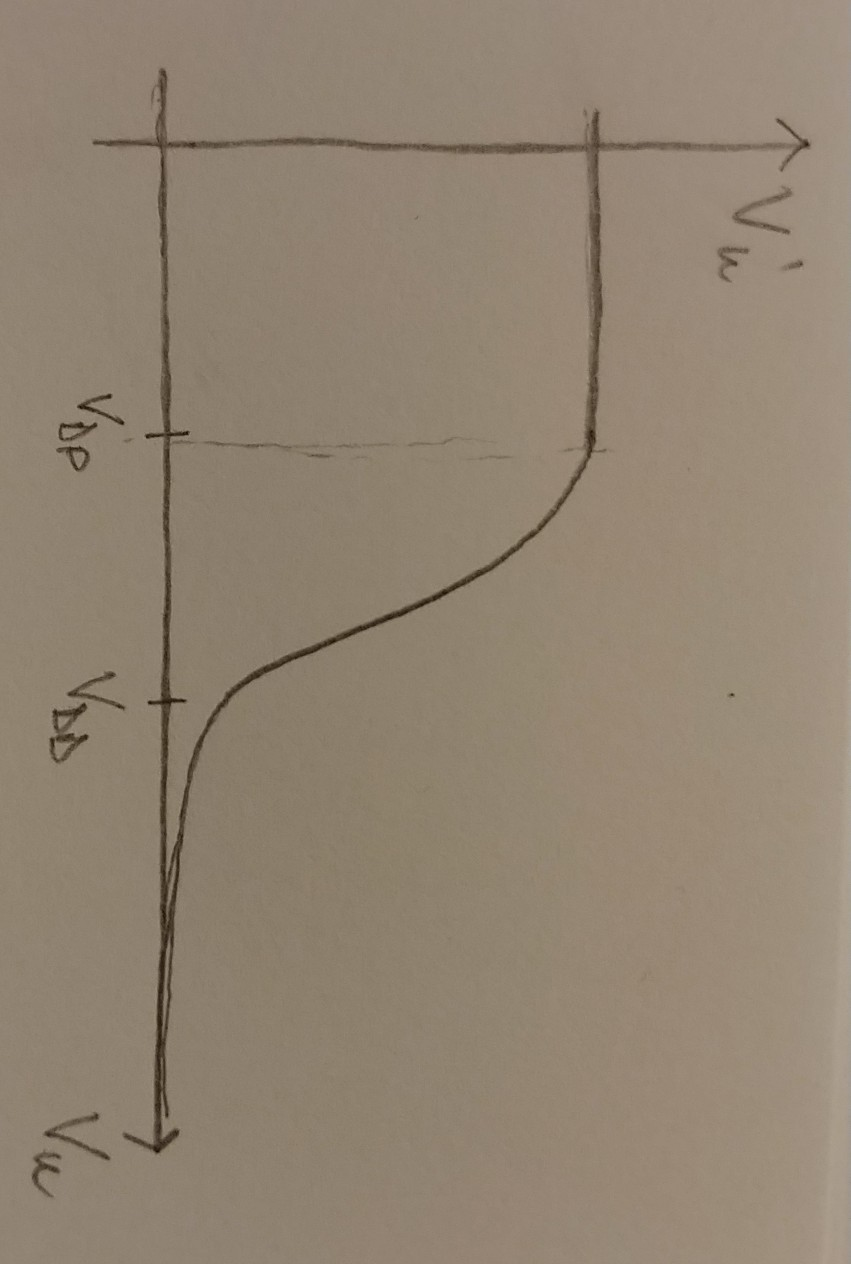
\includegraphics[width=1.8in, angle=90]{img/elettronica/grafico_invertitore.jpg}

    \caption{Grafico invertitore}
\end{figure}

\end{minipage}

Caratteristica a 3 rami:
\begin{itemize}
    \item un ramo estremamente ripido
    \item due rami costanti
\end{itemize}


Cambiando il modo comune $V_{ic}$l'uscita differenziale non cambia

Doppio ingresso ed uscita singola, posso  un segnale in ingresso differenziale, $V_id$ ed un segnale in ingresso in modo comune $V_ic$  (Grafico)



\begin{minipage}{0.5\textwidth}
\begin{figure}[H]
    \centering
    \begin{circuitikz}
        \draw(0, 0) node[left]{$V_i$}
        to[short, i=$I^+{=}0$, *-] ++(1.5, 0)
        node[op amp, anchor=+, yscale=-1](amp){};
        \draw(0, |-amp.-) node[left]{$V_2$} to[short, *-, i=$I^- {=} 0$] (amp.-);
        \draw (amp.out) to[short, -*] ++(0.2, 0)
        node[above]{$V_u$};
    \end{circuitikz}
    \caption{Amplificatore Operazionale}
\end{figure}
\end{minipage}
\begin{minipage}{0.5\textwidth}
\begin{tikzpicture}
    \begin{axis}[axis lines =middle, yticklabels=\empty, xticklabels=\empty,  ymax=3, ymin=-3, xlabel=$V_{id}$, ylabel=$V_u$]
        \addplot[color=red, domain=-4:0, smooth]{-2};
        \addplot[color=red, domain=0:4, smooth]{+2};
        \addplot+[mark=none, color=red, domain=-2:2] coordinates{(0, -2) (0, 2)} ;
    \end{axis}
\end{tikzpicture}
\end{minipage}


Posso definire la pendenza della retta passante per l'origine come $A_d = \frac{dV_U}{dV_{id}} \rightarrow \infty $

Lo chiamo guadagno differenziale perche \'e il guadagno dell'uscita riferito all'ingresso differenziale

Allostesso modo posso definirea anche $A_c = \frac{dV_U}{dV_{ic}}\rightarrow 0$

Possiamo introdurre un parametro di qualit\'a: \textit{CCMR: Common Mode Rejection Ratio}
\[
    \text{CMMR} = \left| \frac{A_d}{A_c}\right|
\]
Idealmente $CMRR \rightarrow \infty$

Chiamata \textbf{Regione di alto guadagno}($AG$) La retta quasi verticale passante per l'origine abbiamo che

\underline{AG}
\[
    V_{id} = 0
\]
\[ -V_n < V_n < +V_n \]

Abbiamo poi due altre regioni, in cui il guadagno \'e nullo, chiamandole rispettivamente $\cdots$

SAT+:
\(
    Vu = V_M
\),
\(
    V_{id} > 0
\)

SAT-:
\(
    Vu = -V_M
\),
\(
    V_{id} < 0
\)

Aggiungendo un criterio di idealit\'a , suppongo che la tensione di uscita $V_u$ non \'e funzione della corrente di uscita $I_u$

Cio\'e $V_u \neq f(I_u)$

$\rightarrow$ Si comporta come generatore di tensione ideale

Le caratteristiche di questo amplificatore sono:
\begin{itemize}
\item corrente di ingresso nulla sui morsetti
\item tensione d'uscita indipendente dalla corrente
    \end{itemize}

    Per ricordare, tra i due ingressi posso immaginare una resistenza che li collega con $R \rightarrow \infty$

    poi  un generatore ideale collegato  a di corrente per $I_u$


\begin{circuitikz}
    \draw(0, 0) node[op amp](am) {};

    \draw(am.-) to[R, l_=$R\rightarrow\infty$, /tikz/circuitikz/bipoles/length=.8cm] (am.+);
    \draw(am.out) -- ++(-0.5, 0)
    to[R, l=$R\rightarrow0$] ++(0, -2)
    to[vsource] ++(0, -1)
    node[eground]{};
    \draw(am.-) to[short, -*] ++(-0.3, 0);
    \draw(am.+) to[short, -*] ++(-0.3, 0);
    \draw(am.out) to[short, -*] ++(+0.3, 0);


\end{circuitikz}

\subsection{Utilizzi}
% altro circuito
Quello che voglio \'e tracciare la caratteristica di trasferimento $V_u$ in funzione di $V_i$

Inizio dalla regione di Auotguadagno:
\[
    \begin{split}
        V_{id} = 0\\
        V_{id} = V^+ - V^- \rightarrow V^- = -V_{id}
    \end{split}
\]

Applicando Kirkoff
\[
    \begin{rcases}
    I_u = \cancel{I^-} + I_2\\
    I_1 = \frac{V_i - \cancel{V^-} }{R_1} = \frac{V_i}{R_i}\\
    I_2 = \frac{V^- - V_u}{R_2}
    \end{rcases}
    \Rightarrow \frac{V_i}{R} = -\frac{V_u}{R_2} \rightarrow V_u = - \frac{R_2}{R_1}V_i
\]

\begin{figure}[H]
    \centering
    
\includegraphics[width=1.8in]{placeholder.jpg}
    \caption{Grafico}
\end{figure}
\[
    V_u = \cancel{-}\frac{R_2}{R_1} V_i = \cancel{-}V_M
\]

Nella zona di \underline{SAT+}:
\[
    \begin{split}
    V_u = +V_M\\
    V_{id} > 0 \\
    V_{id} = V^+ - V^-
    \end{split}
\]

\[
    \begin{rcases}
        I_1 = \frac{V_i - V^-}{R_1}\\
        I_2 = \frac{V^- - V_u}{R_2}
    \end{rcases} \Rightarrow \frac{V_i - V^-}{R_1} = \frac{V^- - V_M}{R_2} \Rightarrow \cdots \Rightarrow
V^- = \frac{R_2 V_i + R_1 V_M}{\cancel{R_1 + R_2}} < 0
\]
\[
    R_2 V_i + R_1 V_M < 0 \Rightarrow \framebox{$V_i < -\frac{R_1}{R_2} V_M$}
\]

La retta \'e lineare $\rightarrow$ \'e un buon amplificatore perch\'e non distorce il segnale

Un altro aspetto importante \'e che quella curva non dipende dai parametri operazionali, dipende unicamente dalle resistenze, \'e totalmente indipendente dalla qualit\'a dell amplificatore stesso

\begin{figure}[H]
\begin{circuitikz}
    \draw (0, 0) node[eground]{}
        to[vsource] ++(0, 2)
        node[above]{$V_i$}
        to[R, -*, l=$R_1$, i=$I_1$] ++(3, 0)
        coordinate(ing1)
        -- ++(0, 1)
        to[R, l=$R_2$, i=$I_2$] ++(3, 0)
        coordinate(tip);
        \draw (ing1) node[op amp, anchor=-](am){};
        \draw(am.+) -- ++(0, -1) node[eground]{};
        \draw(tip) -- (tip |- am.out);
        \draw(am.out) to[short, -o] ++(2, 0) node[above]{$V_u$};
        \draw(am.-) to[open, v>=$V_{id}$] (am.+);
\end{circuitikz}
\centering
\caption{Amplificatore invertente}
\end{figure}

Principio di cortocircuito virtuale: non \'e cortocircuito dal punto di vista della corrente, ma la tensione risulta virtualmente a terra

\underline{AG}
\[
    \begin{rcases}
    \begin{rcases}
        V_{id} = 0\\
        V_{id} = V^+ - V^-
    \end{rcases}
    \Rightarrow V^+ = V^- \rightarrow V^- = V_i\\
    \begin{rcases}
    I_1 = \frac{0 - V^-}{R_1}\\
    I_2 = \frac{V^- - V_U}{R_2}\\
    I_1 = I_2 + \cancel{I^-}
    \end{rcases}
    \end{rcases}\Rightarrow
        \frac{V_i}{R_1} = -\frac{V_u}{R_2} \Rightarrow
    V_u = \frac{R_2}{R_1} V_i
\]
\[
    \text{per} -V_M < V_U < +V_M
\]

\underline{SAT+}
\[
    V_u = +V_M
\]
\bigbreak
\[
    \begin{rcases}
        V_{id} > 0\\
        V_{id} = V^+ - V^-
    \end{rcases}\rightarrow V^+ > V^-
\]
\bigbreak
\[
    \begin{rcases}
    I_1 = \frac{0 - V^-}{R_1}\\
    I_2 = \frac{V^- - V_u}{R_2}
\end{rcases} \rightarrow -\frac{V^-}{R_1} = \frac{V^- - V_M}{R_2} \rightarrow V^-\left(\frac{1}{R_2} + \frac{1}{R_1}\right) = \frac{V_M}{\cancel{R_2}}
\]

\[
    V^- = \frac{R_1}{R_1 + R_2} V_M < V_i
    \Rightarrow \framebox{$V_M < V_i \frac{R_1 + R_2}{R_1}$}
\]
\begin{figure}[H]
    \centering
    \begin{tikzpicture}
        \draw[thick, ->] (-5, 0) -- (5, 0) node[below]{$V_i$};
        \draw[thick, ->] (0, -3) -- (0, +3) node[right]{$V_u$};
        \draw (-4, 2) -- (-1, 2) -- (1, -2) -- (4, -2);
        \draw (-3, 2) node[above]{$Sat+$};
        \draw ( 3, -2) node[above]{$Sat-$};


        \draw (-1, 0) node[circle, fill, label =$-\frac{R_1}{R_2}V_{max}$]{};
        \draw (+1, 0) node[circle, fill, label =$+\frac{R_1}{R_2}V_{max}$]{};
    \end{tikzpicture}

    \caption{Grafico}
\end{figure}

$\Rightarrow$ Tratto orizzontale

\begin{figure}[H]
    \centering
    \begin{circuitikz}
        \draw (0, 0)
        node[above]{$V_i$}
        to[C, *-*, l=$C$, i=$I_C$] ++(2, 0)
        coordinate(ing1)
        -- ++(0, 1)
        to[R, l=R, i=$I_R$] ++(2.5, 0)
        coordinate(tip);
        \draw (ing1) node[op amp, anchor=-](am){};
        \draw(am.+) -- +(0, -1) node[eground]{};
        \draw(am.out) to[short, -*] ++(3, 0)
        node[right] {$V_u$};
        \draw(tip) -- (tip |- am.out);
        \draw(am.-) to[open, v>=$V_{id}$] (am.+);
    \end{circuitikz}
    \caption{Circuito derivatore}
\end{figure}

\underline{AG}
\[
    V_{id} \rightarrow V^+ - V^- = 0 \rightarrow V^- = 0
\]
\[
    \begin{rcases}
        I_c = \cancel{I^-} + I_R\\
        I_c = C \frac{d(V_i- \cancel{V^-})}{dt}\\
    I_R = \frac{\cancel{V^-} - V_u}{R}
    \end{rcases}
    \rightarrow C\frac{dV_i}{dt} = - \frac{V_u}{R} \rightarrow V_u(t) = -RC \frac{dV_i}{dt}
\]
